\chapter{Prototypische Implementierung}
\label{chap:impl}
Dieses Kapitel widmet sich der prototypischen Implementierung der im vorigen Kapitel vorgestellen Konzeption, die als Vorgabe in C++ entwickelt werden muss. Anhand des UML-Klassendiagrammes in \Fref[plain]{fig:uml} wird der grobe Aufbau gezeigt. Als nächster Punkt wird die Abstraktion des Netwerkes erklärt. Danach wird -- ausgehend von der Applikation -- die Implementierung des Publish/Subscribe-Systems erläutert. Angewandte Techniken wie \ac{tmp} oder \emph{policy based}-Design werden im Anhang dieser Arbeit beschrieben. Sie werden benötigt um den zusätzlichen Verwaltungsaufwand zur Laufzeit durch geschickte Anwendung des zur Übersetzungszeit vorhandenen Wissens zu minimieren. Das nutzbare Wissen umfasst zum Beispiel die Typen der Events, die zur Optimierung ausgewählten Strategien und deren Besonderheiten.

\Fref{fig:uml} stellt ein vereinfachtes Klassenmodell des Frameworks dar. Nicht abgebildet sind Datentypen zum Austausch mit den Netzwerkkomponenten oder sonstige Hilfsstrukturen. \emph{P2PInterface} ist eine abstrakte Basisklasse und repräsentiert die in \cite{Dabek2003Towards} beschrieben KBR-API. Aktuell wird diese vom \emph{ChimeraWrapper} implementiert, der über den \emph{ChimeraWrapperImpl} mit dem Netzwerk Chimera spricht. Hier wurde das ``PIMPL''-Pattern angewandt, mit dem die eigentliche Implementierung versteckt werden kann \cite{Alexandrescu2001Modern}. Zur Vereinfachung werden sämtliche Identifikationsdaten, zum Beispiel die Adresse eines Knotens, des Netzwerkes als \emph{std::string} repräsentiert. Dies entbindet den Entwickler der Implementierung weiterer Wrapperklassen. Sollte ein std::string nicht ausreichen um die nötige Information bereitzustellen muss eine Hashmap als weitere Indirektion eingebunden werden. Zur Nachrichtenübertragung wird der Datentyp \emph{std::vector<char>} bereitgestellt, also die objektorientierte Version eines \emph{char*}. Dies bietet zusätzlichen Schutz gegen Bufferüberlauf oder ähnliche Probleme.\\
Für weitere Netzwerke können auf einfache Art und Weise Wrapperklassen geschrieben und eingebunden werden.

\begin{figure}[htbp]
\centering
\resizebox{\textwidth}{!}{%
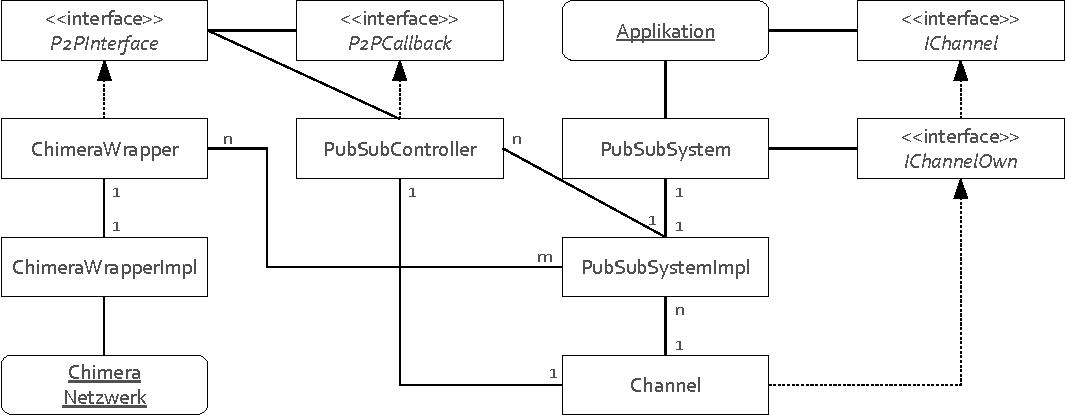
\includegraphics{grafics/uml.pdf}}
\caption{vereinfachtes Klassendiagramm des Frameworks}
\label{fig:uml}
\end{figure}



Die \emph{Applikation} spricht mit dem Singleton \emph{PubSubSytem}, beide können den \emph{Channel} nur über die abstrakte Basisklasse \emph{IChannel} beziehungsweise \emph{IChannelOwn} ansprechen. Durch diese beiden Basisklassen wird die Komplexität der durch Policies optimierten Klasse Channel verdeckt. Der Channel ist eine Templateklassen mit Policies\footnote{siehe \Fref{chap:impl_tmp} im Anhang zur Erklärung}. Die verschiedenen Strategien -- in \Fref{fig:uml} ebenfalls nicht dargestellt -- werden benutzt um den Channel zu spezialisieren. Durch \ac{tmp} ist es weiterhin möglich jeden Channel auf die gewählten Policies abzustimmen. Zur Übersetzungszeit wird zum Beispiel unbenötigter Code entfertn. Weiterhin wird ein optimierten Header erzeugt, dessen Größe an Nutzlast von den von den gewählten Policies abhängig ist. Durch diese Maßnahmen wird der Overhead zur Laufzeit stark reduziert. 

Die Klasse \emph{PubSubController} implementiert das Interface \emph{P2PCallback} und kann sich somit für die Callbacks des Netzwerkes registrieren. Weiterhin bietet diese Klasse die von Channel benötigte Funktionalität. \emph{PubSubSystemImpl} kennt die Netzwerkwrapperklassen (in \Fref{fig:uml} ChimeraWrapper) und verbindet diese über den PubSubController mit dem Channel. Mit verschiedene Instanzen des PubSubControllers können somit auch verschiedene Netzwerke angesprochen werden und entsprechend der Optimierung für verschiedene Channel eingesetzt werden.


\subsection{PubSubabstraktion}
\begin{itemize*}
\item PubSubController spricht mit Netzwerk
\item PubSubSystem spricht mit Applikation und leitet Anfragen an Channel weiter
\item Channel nutzt Controller zum Netzwerkzugriff
\item $\rightarrow$ Möglichkeit verschiedene Netzwerke zu nutzen!
\end{itemize*}

\subsection{Optimierungsschritt}
\begin{itemize*}
\item komplett: ChannelList
\item komplett: PubSubSystemImpl
\item teilsweise: PubSubSystem
\end{itemize*}

\lstinputlisting[caption={Zugriff auf M$^2$etis aus Benutzersicht}, label=lst:pubsub_usage]{listings/pubsub_usage.cpp}


